\documentclass[../main/TOP_manual]{subfiles}

\begin{document}

\chapter{TOP structure and workflow}
\label{chap:ModDes}

TOP is the NEMO hardwired interface toward biogeochemical models, which provides the physical constraints/boundaries for oceanic tracers (Fig. ~\ref{fig:topstructure}).

Based on a modular structure, this component allows one to exploit available built-in modules and further develop a range of applications, spanning from the implementation of a dye passive tracer to evaluate dispersion processes (by means of MY\_TRC), track water masses age (AGE module), assess the ocean interior penetration of persistent chemical compounds (e.g., gases like CFC or even PCBs), up to the full set of equations to simulate marine biogeochemical cycles.

TOP interface has the following location in the code repository : \path{<nemo-repository>/src/TOP/}

and the following modules are available:

%-----------  tableau  ------------------------------------
\begin{itemize}
        \item \textbf{TRP}    	 :    Interface to NEMO physical core for computing tracers transport
        \item \textbf{CFC}	 :    Inert tracers (CFC11,CFC12, SF6)
        \item \textbf{C14}	 :    Radiocarbon passive tracer
        \item \textbf{AGE}	 :    Water age tracking
        \item \textbf{MY\_TRC}   :    Template for creation of new modules and external BGC models coupling
        \item \textbf{PISCES}    :    Built in BGC model. See \cite{aumont_2015} for a complete description
\end{itemize}
%----------------------------------------------------------

\begin{figure}[ht]
\begin{center}
\vspace{0cm}
\includegraphics[width=0.70\textwidth]{Fig_TOP_design}
\caption{Schematic view of the TOP interface within NEMO framework}
\label{fig:topstructure}
\end{center}
\end{figure}

\pagebreak

% the following figures are screenshot of the mermaid plot genereted when accessing TOP/figures/workflow.md within gitlab
% this plots should be rewritten, e.g., using tikz graphic package

The workflow of the TOP interface within the NEMO framework is organized around two main blocks of the code, the initialization (\autoref{fig:topinit}) and time marching or "stepping" (\autoref{fig:topstep}) procedures.\\

The initialization (\forcode{trc_init}) of passive tracers variables and parameters include reading namelist, set initial tracer fields (either read restart or read data), and specific initialisation for each SMS module.

\begin{figure}[ht]
\begin{center}
\vspace{0cm}
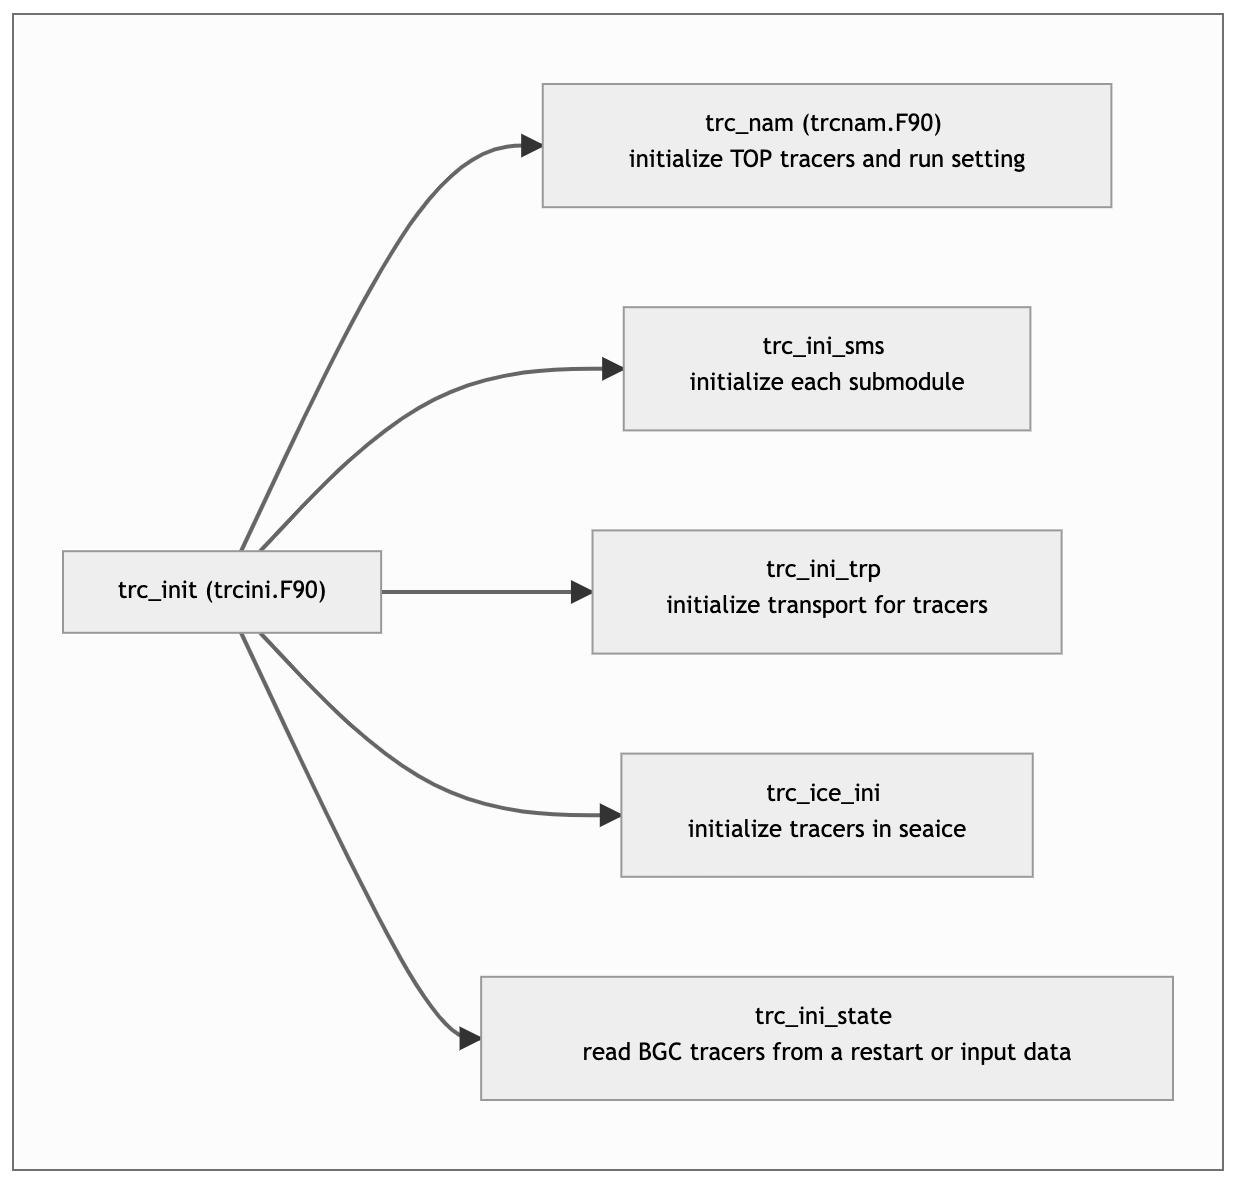
\includegraphics[width=0.75\textwidth]{TOP_init}
\caption{TOP interface initialization workflow (called by nemo\_ini in \forcode{OCE/nemogcm.F90})}
\label{fig:topinit}
\end{center}
\end{figure}

In the time-marching procedure of the model (trc\_stp), trends are computed for all tracers in relation to biogeochemical processes (source minus sinks of each TOP sub-module), 
physical transport (advective \& diffusive, forcing and boundary conditions) and output is managed using the I/O library XIOS.

\begin{figure}[ht]
\begin{center}
\vspace{0cm}
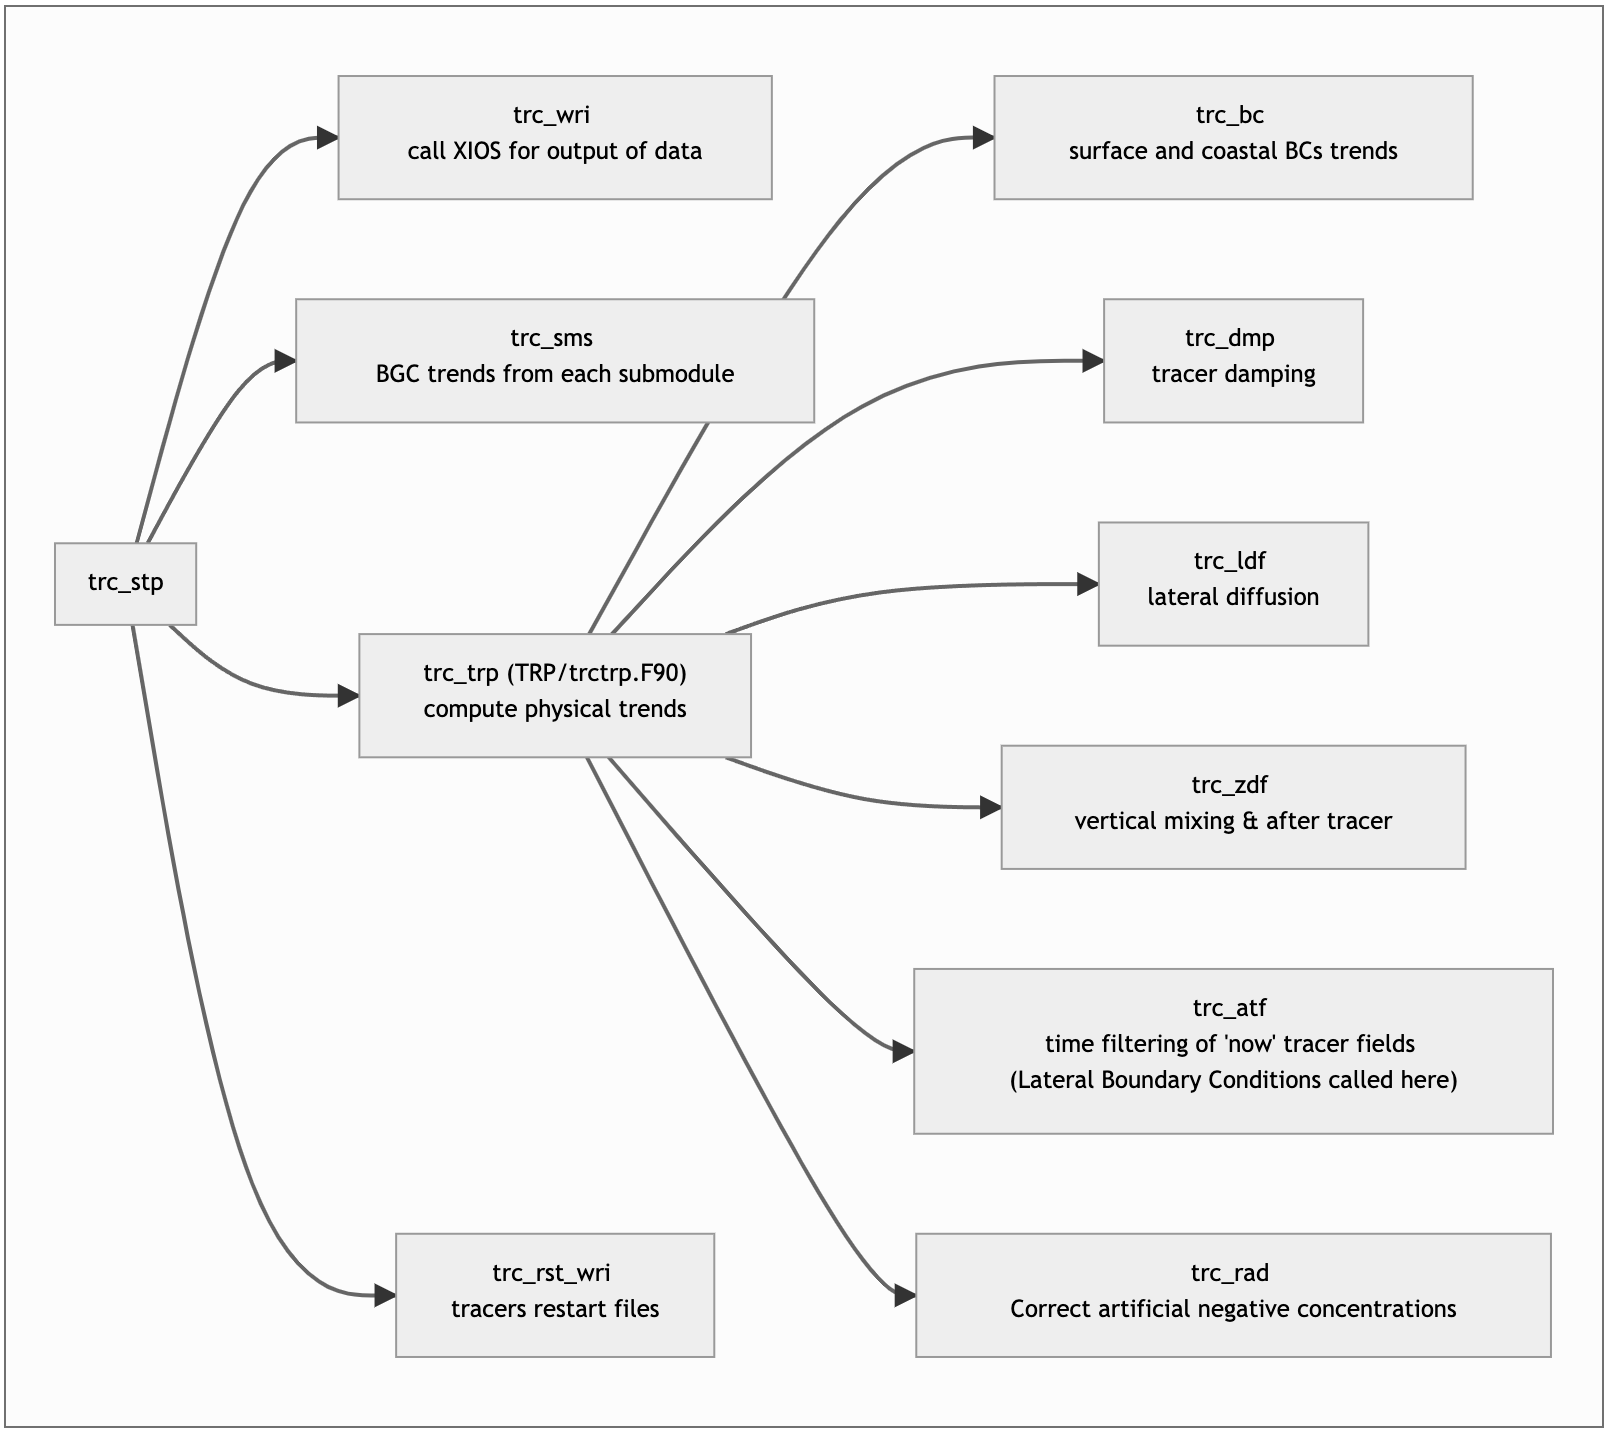
\includegraphics[width=0.75\textwidth]{TOP_step}
\caption{TOP interface time-marching workflow (called by stp in \forcode{OCE/step.F90}}
\label{fig:topstep}
\end{center}
\end{figure}

\end{document}
